\documentclass[a4paper, twocolumn]{article}
\setlength{\textwidth}{180mm}
\setlength{\textheight}{250mm}
\setlength{\parindent}{0mm}
\setlength{\parskip}{2mm}
\setlength{\oddsidemargin}{15mm}
\setlength{\hoffset}{-1in}
\setlength{\topmargin}{-2.5pc}
\setlength{\headsep}{20pt}
\setlength{\columnsep}{4mm}
\usepackage{amsmath}
\usepackage{graphicx}
\usepackage{listings}
\lstset{
    language=C, 
    literate={\ \ }{{\ }}1, 
    keywordstyle=\bfseries, 
    basicstyle=\ttfamily}
\def\ttdefault{pcr}
\begin{document}
\section*{Foreword}
I used the \verb!c! programming language to complete this task. I %
represented the system of spins as a \verb!struct!, %
defined below in one dimension. 

\begin{lstlisting}
typedef struct ising_t
{
    float epsilon;
    float magnetic_field;
    float epsilon;
    int length;
    int *ensemble;
} ising_t;
\end{lstlisting}

Scaling this to two dimensions was more difficult because the %
\verb!*ensemble! had to be transformed into \verb!**ensemble!. %
It is possible to implement this in a single \verb!struct! %
using \verb!union ensemble {int *1d, int **2d};!, but in the %
code available on my \verb!github! I have used two separate %
\verb!struct!s resulting in code duplication for many of the %
methods. I made this decision because I had not used \verb!c! %
prior to this project and was unaware of the \verb!union! %
keyword and its uses. I am describing this because you may %
notice discrepancies in the code snippets that I have include %
where \verb!int *(*)ensemble = system -> ensemble;! is invoked %
to access the array of spins. 


\subsection*{Question 1 a)}
I selected three different temperatures, \(1.0, 2.0\) and %
\(3.0 \epsilon / k\), and ran the metropolis algorithm for %
\(1000N\) steps. At each of these temperatures the system %
was initialised in a random state and allowed to equilibrate. 

\begin{figure}[h]
    \includegraphics%
        [width=0.45\textwidth]%
        {pub/figures/first_and_last_ising_1d.pdf}
    \caption{Each vertical pair of lines %
        represents the spin state. The top one is %
        the random initial state and the bottom one %
        is the equilibrated final state.}
    \label{fig:1}
\end{figure}

We noticed that at lower temperatures the spin chunks were %
much larger than at higher temperatures. This is particularly %
pronounced between the \(T = 3.0\epsilon/k\) and \(T = %
1.0\epsilon/k\) plots in figure \ref{fig:1}. To evolve the %
system we used the version of the metropolis algorithm %
shown below, 

\begin{lstlisting}
/*
 * metropolis_step
 * ------------------------ 
 * Evolve the system by attempting to 
 * flip a spin. The step is weighted 
 * by the Boltzmann factor.
 *
 * parameters
 * ----------
 * ising_t *system: A struct 
 *     enscapulating the information 
 *     related to the system. 
 */
void metropolis_step(ising_t *system)
{
    float temp = system -> temperature;
    int *ensemble = system -> ensemble;
    int length = system -> length;
    int spin = random_index(length);
    int change = 2*ensemble[spin]*(
        ensemble[modulo(spin+1,length)] +
        ensemble[modulo(spin-1,length)]);

    if ((change < 0)
        || (exp(-change/temp)>randn()))
    {
        ensemble[spin] *= -1;
    }
}
\end{lstlisting}

where, \verb!rand! generates a random number in the range %
\([0, 1]\), and \verb!modulo! is modified to produce %
positive input on negative numbers like the \verb!python! %
implmentation. This is not the native \verb!c! implementation. %
I used the \verb!||! short circuit operator so that %
the second comparison was not evaluated on every call %
to the function. 
            

\subsection*{Question 1 b)}
I found that it was worth considering what the \emph{basic %
unit} of the Ising model was. In the absence of an external %
magnetic field the energy is a function of the pairs. I start %
by considering the partition function of an individual pair. %
This is a two level system; either the pair are aligned or they %
are anti-aligned with the corresponding energies.
%
\begin{align}
    Z_{i} &= \sum_{s_{i} = \pm 1}
            \exp\left(-\frac{\varepsilon s_{i}s_{i+1}}{\tau}\right)
            \nonumber\\
        &= \exp\left(-\frac{\varepsilon}{\tau}\right) +
            \exp\left(\frac{\varepsilon}{\tau}\right)
            \nonumber\\
        &= 2\cosh\left(\frac{\varepsilon}{\tau}\right).
    \label{eqn:1}
\end{align}


Similarly to the para-magnetic case we can multiply the system %
partition functions of single constituents together to get the %
partition function of the entire system. However, the condition %
to do this was that the constiutuents were independent, but the %
Ising model contains interactions. In the case of the Ising model %
the constituents that are independent are the pairs, not the %
individual spins. You may think think then that we only consider %
\(N / 2\) unique pairs but this is not the case. In a chain each %
spin is counted in two pairs so the power is still \(N\). 


A small detail that I skipped was what happens at the boundary. %
The two spins on the end of the chains are not (neccessarily) %
counted twice. In the limit of a very large chain of spins we %
can see that the boundary affect will not matter however, we %
got about this nuance in a much more interesting way by considering %
cyclic boundary conditions. That is to say that the spin on the %
far end of the chain is a neighbour to the spin at the start of the %
chain and vice versa. 


Given the partition function \(Z = (2\cosh(\varepsilon / \tau))^{N}\), we 
calculated the internal energy using,

\begin{align}
    U &= \tau^{2}\partial_{\tau}\ln(Z)\label{EQN1}\\
        &= \tau^{2}\partial_{\tau}
            \ln\left(2\cosh\left(\frac{\varepsilon}{\tau}\right)^{N}\right)
            \nonumber \\
        &= N\tau^{2}\partial_{\tau}
            \ln\left(2\cosh\left(\frac{\varepsilon}{\tau}\right)\right)
            \nonumber \\
        &= N\tau^{2}\partial_{\tau}
            \left(2\cosh\left(\frac{\varepsilon}{\tau}\right)\right)
            \frac{1}{2\cosh\left(\frac{\varepsilon}{\tau}\right)}
            \nonumber \\
        &= N\tau^{2}\partial_{\tau}\left(\frac{\varepsilon}{\tau}\right)
            \frac{\sinh\left(\frac{\varepsilon}{\tau}\right)}
            {\cosh\left(\frac{\varepsilon}{\tau}\right)}\nonumber \\
        &= -\varepsilon N\tanh\left(\frac{\varepsilon}{\tau}\right)
    \label{eqn:2}.
\end{align}

We calculated the free energy of the system using,

\begin{align}
    F &= -\tau\ln Z \\
        &= -\tau\ln\left(\left(
            2\cosh\left(\frac{\varepsilon}{\tau}\right)\right)^{N}\right) 
            \nonumber \\
        &= -N\tau\ln\left(
            2\cosh\left(\frac{\varepsilon}{\tau}\right)\right) 
            \nonumber \\
        &= -N\tau\ln\left(
            \exp\left(\frac{\varepsilon}{\tau}\right) + 
            \exp\left(-\frac{\varepsilon}{\tau}\right)\right) \nonumber \\
        &= -N\tau\ln\left(\exp\left(\frac{\varepsilon}{\tau}\right)
            \left(1 + \exp\left(-2\frac{\varepsilon}{\tau}\right)\right)
            \right)\nonumber \\
        &= -N\tau\ln\left(\exp\left(\frac{\varepsilon}{\tau}\right)\right)
            - N\tau\ln\left(1 + 
            \exp\left(-2\frac{\varepsilon}{\tau}\right)\right) \nonumber \\
        &= -N\varepsilon - N\tau\ln\left(1 + 
            \exp\left(-2\frac{\varepsilon}{\tau}\right)\right)
    \label{eqn:3}. 
\end{align}

The entropy followed from the combination of Equation \ref{eqn:2} and %
Equation \ref{eqn:1} using Equation \ref{eqn:3},

\begin{align}
    \tau\sigma &= F - U\\
        &= -N\varepsilon\tanh\left(\frac{\varepsilon}{\tau}\right) + 
            N\varepsilon + N\tau\ln\left(1 + 
            \exp\left(-2\frac{\varepsilon}{\tau}\right)\right)\nonumber \\
    \sigma &= \frac{\varepsilon}{\tau}\left(1 - 
            \tanh\left(\frac{\varepsilon}{\tau}\right)\right) +
            \ln\left(1 + \exp\left(-2\frac{\varepsilon}{\tau}\right)\right)
    \label{eqn:4}.
\end{align} 

Finally, we determined the specific heat using Equation \ref{eqn:2} %
and Equation \ref{eqn:3},

\begin{align}
    C &= \partial_{\tau}U\\
        &= \partial_{\tau}\left(-N\varepsilon\tanh\left(
            \frac{\varepsilon}{\tau}\right)\right)\nonumber\\
        &= -N\varepsilon\partial_{\tau}\left(\frac{\varepsilon}{\tau}\right)
            \frac{1}{\cosh^{2}\left(\frac{\varepsilon}{\tau}\right)}
            \nonumber\\
        &= \frac{N\varepsilon^{2}}{\tau^{2}\cosh^{2}\left(
            \frac{\varepsilon}{\tau}\right)}
    \label{eqn:5}.
\end{align}    


\subsection*{Question 1 c)}
\begin{figure}[h]
    \centering
    \includegraphics%
        [width=0.45\textwidth]%
        {pub/figures/physical_parameters_ising_1d.pdf}
    \caption{The top left is the energy and the %
        top right is the entropy. The bottom left is the %
        free energy and the bottom right is the heat capacity.}
    \label{fig:2}
\end{figure}        

I started by simulating a one dimensional Ising model with no %
external magnetic field, which I compared to the analytic %
expressions derived above. I used periodic boundary conditions %
and chose to implement my models using a lattice size of one-hundred %
spins. I chose to use one-hundred spins because it evaluated %
fast on my device and was large enough to be interesting. 


Starting with our one dimensional model we equilibrated the %
system for multiple different temperatures and settled on %
using \(1000N\) as the length of the loop. This was likely %
too many but I found that for low temperatures when the %
probability of a flip becomes small, a larger number of %
steps was required. 


I chose to sample the temperatures over the range \(0.0 - 4.0 %
\epsilon / k\) incrementing by \(0.2 \epsilon / k\). I %
initialised the system only once at the highest temperature %
that we sampled, \(3.8 \epsilon / k\). I equilibrated the %
system at this temperature by evolving it for \(1000N\) %
and then started to cool the system taking measurements %
at each new system. 


The alternative model was to randomly initialise the system %
at every temperature. This would require approximately %
twice the number of steps since the system would have to %
be equilibrated at every temperature. I realize that the %
cooling method has a side affect of leading to "overflow". %
By "overflow" I mean that the first few measurements of %
each temperature are slightly out of equilibrium at the %
higher temperature. 


The entire \emph{measured} cooling process was performed %
by the program \(1000\) times. At each temperature in the %
\emph{measured cooling} loop the energy and entropy %
were measured by taking the average of all \(1000 N\) %
iterations. The heat capacity was also measured by taking %
the variance of the energy and applying,
%
\begin{equation}
    C_{v} = \frac{\textrm{var}(\epsilon)}{\tau^{2}}
    \label{eqn:6}
\end{equation}


The energy and entropy were re-averaged over the outer %
\emph{fixed size} loop. I chose to re-average then on %
the outer loop because I was certain that the trials were %
statistically independent. This does not matter so much %
for the mean value estimate since the \(1000N\) inner %
loop allows the system to explore the equilibrium space %
but I think that it does matter for the error estimate. 


I belive that it matters for the error estimate because %
the state of the system is highly correlated to the %
past state of the system within some \emph{correlation %
length}. This \emph{correlation length} is roughly the %
same amount of time that the system requires to explore %
the equilibrium state, or \(1000N\).


By running multiple simulations for the \emph{correlation %
length} and averaging these results I have guaranteed %
robust results. I estimated the error using the \emph{standard %
error} of the independent \emph{correlation length} simulations. %
This means that the error presented in figure \ref{fig:2} is %
given by equation \ref{eqn:7}.
%
\begin{equation}
    \Delta\hat{\beta} = \sqrt{\frac{\textrm{var}(\beta)}{N}},
    \label{eqn:7}
\end{equation}
%
where, \(\hat{\beta}\) is the parameter estimate, \(\beta\) is a %
vector of measurements and \(N\) is the number of measurements. 


To calculate the energy of the system I used the following %
algorithm, 

\begin{lstlisting}
/*
 * energy_ising_t
 * --------------
 * Calculate the energy of the system.
 *
 * parameters
 * ----------
 * ising_t *system: A struct 
 *     enscapulating the information 
 *     related to the system. 
 *
 * returns
 * -------
 * float energy: The energy of the
 *     system in Joules. 
 */
float energy_ising_t(ising_t *system)
{
    int length = system->length;
    int *ensemble = system->ensemble;
    float energy = 0.;

    for(int spin=0; spin<length; spin++)
    {
        energy -= ensemble[spin] *  
            ensemble[modulo(spin+1,length)];
    }

    return energy;
}
\end{lstlisting}


You may notice that I am only counting the righthand neighbour %
of each spin. I chose this method because it is more optimal. %
If I was to count each neighbour then every pair would be %
counted twice and we would have to divide the final result by %
\verb!2.!. By only counting one of the neighbours I have %
halved the number of computations. 


A pair of spins is the \emph{base unit} of the ising model %
so to calculate the entropy I counted the number of aligned %
pairs and then used the \emph{chose} function to calculate %
the multiplicity. However, it was not quite this simples %
since \(100!\) is \(\sim 10^{157}\), which overflows an %
integer in the programs memory. 


To fix this problem I used the stirling approximation to %
compute the entropy directly. This implies that the %
entropy should be less accurate at lower temperatures %
where the entropy is low and the Stirling approximation %
diverges from the actual entropy. The code that I used %
to calculate the entropy was,

\begin{lstlisting}
/*
 * entropy_ising_t
 * ---------------
 * Calculate the entropy of a 
 * configuration. 
 *
 * parameters
 * ----------
 * ising_t *system: A struct 
 *     enscapulating the information 
 *     related to the system. 
 *
 * returns
 * -------
 * float entropy: The entropy of the
 *     system in natural units. 
 */
float entropy_ising_t(ising_t *system)
{ 
    int length = system->length;
    int *ensemble = system->ensemble; 
    int up = 0;

    for (int spin=0; spin<length; spin++)
    {
        up += ensemble[spin] == 
            ensemble[modulo(spin+1,length)];
    }

    int down = length - up;

    float entropy = length * log(length) - 
        up * log(up) - down * log(down);
    
    return entropy;   
}
\end{lstlisting}


\subsection*{Question 1 d)}
Consider the energy depicted in figure \ref{fig:2}. We see that %
the energy is a decreasing function of the temperature. This %
implies that the spins tend to align as the temperature decreases. %
This makes sense because the Boltzmann factor for the lower state %
becomes more favoured. Similarly the entropy is a increasing %
function of the temperature. As the spins tend to align at lower %
temperatures the number of ways to arrange the state becomes %
smaller, decreasing the entropy. 


The heat capacity, also shown %
in figure \ref{fig:2} is interesting because it increases %
rapidly before asymptotically decreasing. If it was discontinuous %
then we would expect a phase transition however it is continuous. %
so we know that there is no phase transition. We know it is continuous %
because of equation \ref{eqn:5}. 


\subsection*{Question 1 e)}
\begin{figure}[h]
    \centering
    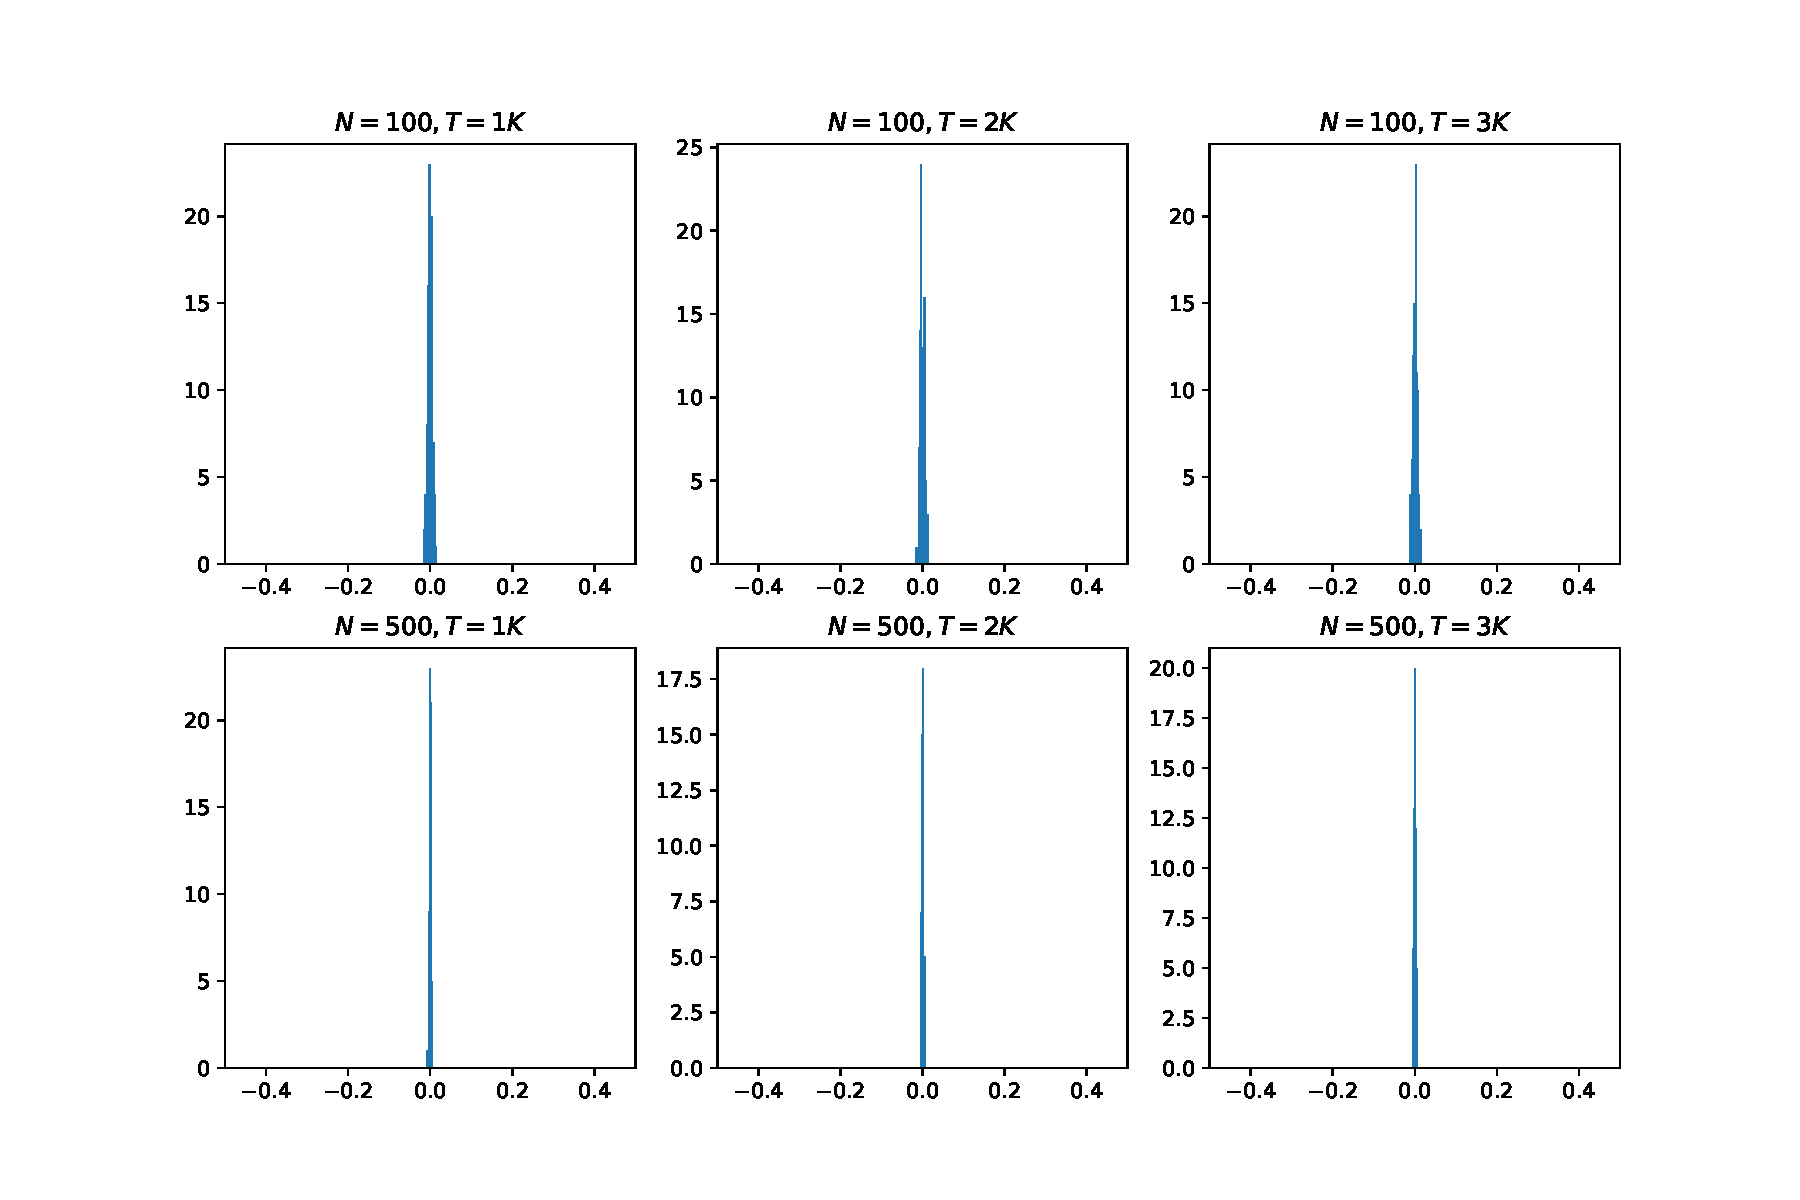
\includegraphics[width=0.45\textwidth]{pub/figures/magnetisation_ising_1d.pdf}
    \caption{Histograms of the magnetisation for two ising %
        systems of sizes \(N = 100\) and \(N = 500\). The %
        temperatures are labelled in the titles and the %
        \(y\)-axis is a unitless count.}
    \label{fig:3}
\end{figure}


Figure \ref{fig:3} showed me that the magnetisation was not zero %
as it was predicted to be at \(0 \epsilon / k\). I am not concerned %
because the distribution of samples, which roughly corresponds to %
a time average is symmetrically distributed around zero implying %
that the time average is identically zero. I would expect some %
variation of the results around zero as spins randomly flipped. %


Since magnetisation sets in at a lower temperature for the larger %
sample I concluded that there was no phase transition. I %
decided this because the phase transition should occur at the %
same temperature for all lattice sizes. Taking the limit of %
a decreasing function presumably reduces to zero implying that %
there is no spontaneous magnetisation for the one-dimensional %
Ising model. This means that there is no phase transition. 


\subsection*{Question 2 a)}
For \(\tau = 1.0 \epsilon / k\) the random lattice very quickly %
relaxed into large \emph{domains} of up and down spins. Over time %
the boundaries of the \emph{domains} moved around the lattice %
coherently. I am/will using/use \emph{coherent motion} to refer %
to a blob transporting across the network. For example, a group %
of down spins may start in the top right corner and remaining %
a single blob move to the middle of the system. 


I noticed that given enough time the \(\tau = 1.0 \epsilon / k\) lattice %
relaxed until it was entirely one color. This is not shown in figure %
\ref{fig:4} simply because the lattice was not allowed to evolve %
for enough time. I used the same evolution time for the two %
dimensional Ising model that I used for the one dimensional %
Ising model, that is \(1000N^{2}\) where I will use \(N\) to %
represent the side length of the system. 


This is important because at lower temperatures the system took longer %
to equilibrate. As I saw for the one-dimensional case the %
\emph{coherent domains} have a \emph{meta-stable} lifetime before decaying. %
The shape of this domain influences the lifetime. The size %
seems to be a direct predictor of lifetime with the largest %
domain nearly always coming out on top. Another important %
feature that we noticed was that the coherent domains became %
particularly \emph{meta-stable} if they formed rings. 


The ring structures were \emph{meta-stable} because of the cyclic %
boundary conditions. In a ring structure there are only two edges %
that are exposed to the other \emph{meta-stable} state meaning %
that the anti-aligned interactions at the boundary are minimised. %
Additionally since the interaction depth of the Ising model is %
only nearest neighbour the \emph{meta-stable} ring could exit %
in a band of just five spins. \emph{The spins on the boundary %
have no idea how large their respective domains are}.


A final point to address for the \(\tau = 1.0\epsilon / k\) model %
is the \emph{time speckling}. As the system is allowed to evolve %
in equilibrium spins at random locations will randomly flip. %
This is a byproduct of the metropolis algorithm but it is important %
because the \emph{speckles} almost always remain a single spin. %
You will see later that this changes as the temperature is increased. 


Heating the lattice to \(\tau = 2.0 \epsilon / k\) we see mush %
of the same behaviour. \(\tau = 2.0 \epsilon / k\) is still less %
than the critical temperature, so all of the same evolutionary %
events occur. \emph{Meta-stable} domains form, move and die. %
Even the more dangerous \emph{meta-stable} rings can form at %
this temperature. I would like to say that the lifetime of the %
\emph{domains} has declined but I have no evidence. 


The key difference between the \(\tau  2.0 \epsilon / k\) and the %
\(\tau = 1.0 \epsilon / k\) models is the \emph{speckling}. At %
the higher temperatures the speckles occur more often and can %
result in very local short lived domains. This is why I postulated %
that the \emph{domains} are shorter lived. The system is more %
active meaning that the spins on the boundary flip more readily. %
Moreover, the rapid speckling assists in the destruction of the %
\emph{domain} when it occurs on the boundary.


Something worthy of note before we move above the condensation %
temperature is that \emph{domains} die at there corners. This %
is because the corners represent an interface where a spin has %
more neighbours of one color than the other. This is another %
factor that prolongs the life of the \emph{meta-stable} states, %
since they have no corners and minimised contact. 


The behaviour was markedly different for the \(\tau = 3.0 \epsilon %
\ k\) model, because it is above the critical temperature. %
For starters the activity of the system has increased significantly. %
This means, among other things that the relaxation into equilibrium %
is almost instantaneous compared with the lower temperature models. %
In addition \emph{domains} do not form at this temperature. 


I have been using \emph{domain} to refer to a structure that is %
\emph{macroscopic} and \emph{semi-permanent}. \emph{Zonation} %
does occur at \(\tau = 3.0 \epsilon / k\) bur it does not meet %
these criteria. By this I mean that the zones are small \(\sim 10\) %
spins maximum and temporary. Rather than considering the rapid %
zonation to be the evolution of the \emph{domain} behaviour I %
consider it the evolution of the \emph{speckling} behaviour.


At \(\tau = 3.0 \epsilon / k\) we also loose the \emph{coherent} %
end state. At both of the other temperatures the final state was %
a completely magnetised block or a \emph{meta-stable} ring. %
However, at \(\tau = 3.0 \epsilon / k\) there is no such state %
and the \emph{zonation} appears to randomly move about the grid. %
At higher temperatures still the \emph{zonation} is completely %
destroyed and not even microscopic domains are able to form. 


\begin{figure}
    \centering
    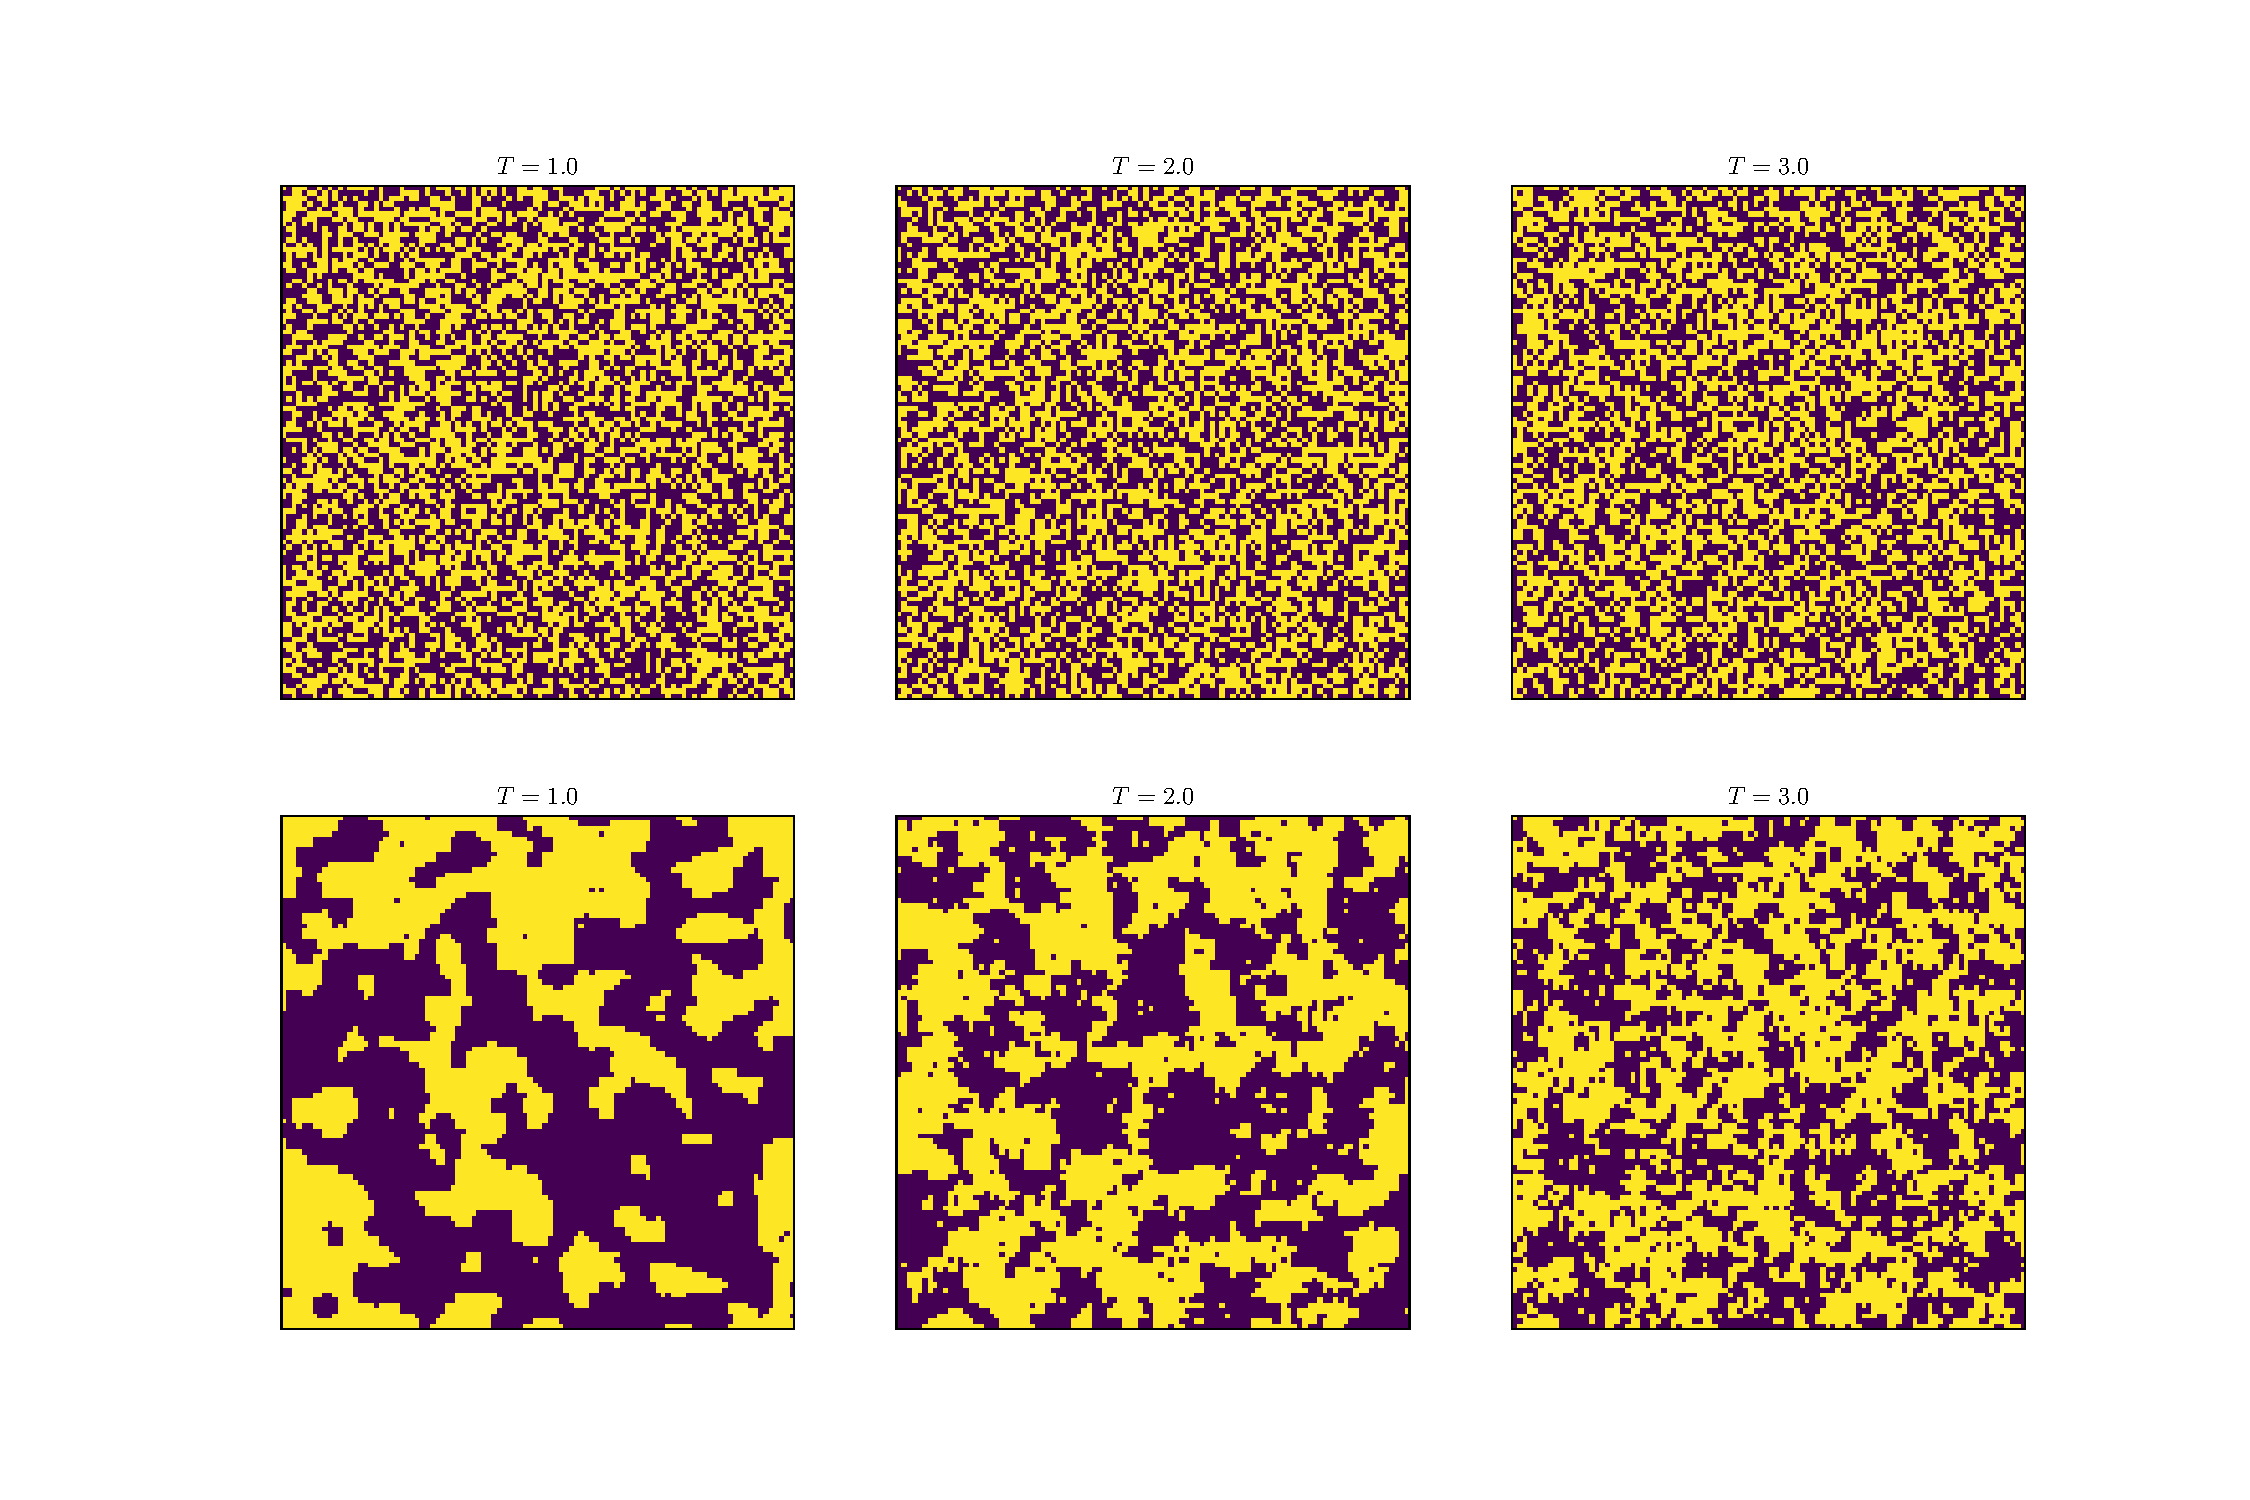
\includegraphics[width=0.45\textwidth]{pub/figures/first_and_last_ising_2d.pdf}
    \caption{Snapshots of the Ising system at multiple temperatures %
        given a random initial starting position (top). You will %
        notice that \(\tau = 1.0 \epsilon / k\) and \(\tau = 2.0 \epsilon %
        /2\) have similar net magnetisation, but that \(\tau = 2.0 %
        \epsilon / k\) has stronger \emph{speckling} than \(\tau = %
        1.0 \epsilon / k\). You will notice that there is not net %
        magnetisation for \(\tau = 3.0 \epsilon / k\) and that the %
        \emph{zonation} I described above is occurring.}
    \label{fig:5}
\end{figure}


\subsection*{Question 2 b)}
Smoothly varying the temperature using I found that the \emph{speckling} %
and \emph{zonation} seems to dominate above \(\sim 2.3 \epsilon / k\) %
while below this \emph{domains} start to form and given enough time %
the entire crystal becomes magnetised. The transition is smooth %
with respect to the \emph{speckles}, which at very low temperatures %
are very small and isolated with out a lifetime. 


As I increased the temperature the \emph{speckles} increases in size and %
in lifetime. A \emph{speckle} is differentiated from a \emph{zone} rather %
arbitrarily, the two main differences being transport and lifetime. The %
\emph{zones} have a lifetime of long enough that they are able to %
\emph{coherently move} across the crystal. On the other hand a \emph{speckle} %
tends to die where it started and very quickly. 


As we approach the critical temperature from below the \emph{speckles} %
increase in size and disrupt the domains more quickly but, the system %
is still able to fully magnetise. At the critical temperature the %
\emph{speckles} become so disruptive that the magnetisation cannot occur %
macroscopically but it still occurs locally in the form of the \emph{zones} %
which outlive the now very active \emph{speckles}. 


Increasing the temperature further still the coherent \emph{zones} %
disappear (visually) entirely and the speckles become the dominant %
behaviour. As a final note it is worth noting that these behaviours %
I have described were visible to me in part because of the settings %
of my simulation. I found it was best to run them with many steps %
per frame \(5000 \sim 10000\) because it allows you to see the %
macroscopic behaviours. 


I acknowledge that although I wanted to use the \verb!qt! frame work %
to create my own \verb!gui! I ran out of time. Instead I used the %
free online applet created by Daniel V. Schroeder for Weber state %
university to make the higher level observations. The code that I used %
to evolve the two dimensional system was, 

\begin{lstlisting}
/*
 * metropolis_step_ising_t
 * -----------------------
 * Evolve the system according to a 
 * randomly weighted spin flip that 
 * compares the probability of the 
 * two states based on the Boltzmann 
 * distribution of the two systems. 
 *
 * parameters
 * ----------
 * ising_t *system: The system to 
 *     evolve. 
 */
void metropolis_step(ising_t *system)
{
    int length = system->length;
    int **ensemble = system->ensemble;
    float epsilon = system->epsilon;
    float temp = system->temperature;
    float field = system->magnetic_field;

    int row = random_index(length);
    int col = random_index(length);

    int spin = ensemble[row][col];
    int neighbours = 
        ensemble[modulo(row+1,length)][col] + 
        ensemble[modulo(row-1,length)][col] + 
        ensemble[row][modulo(col+1,length)] + 
        ensemble[row][modulo(col-1,length)];

    float magnetic_change=-2*spin*field;
    float interaction_change=2*epsilon*
        neighbours*spin;
    float change=magnetic_change+
        interaction_change;

    if ((energy_change < 0) || 
        (exp(-change/temperature) > randn())))
    {
        ensemble[row][col] *= -1;
    }
}
\end{lstlisting}


\textbf{Note}: The \verb!magnetic_field! was set to zero in the %
provided simulation and discussion, while the \verb!epsilon! %
was set to one. 


\subsection*{Question 2 c)}
\begin{figure}
    \centering
    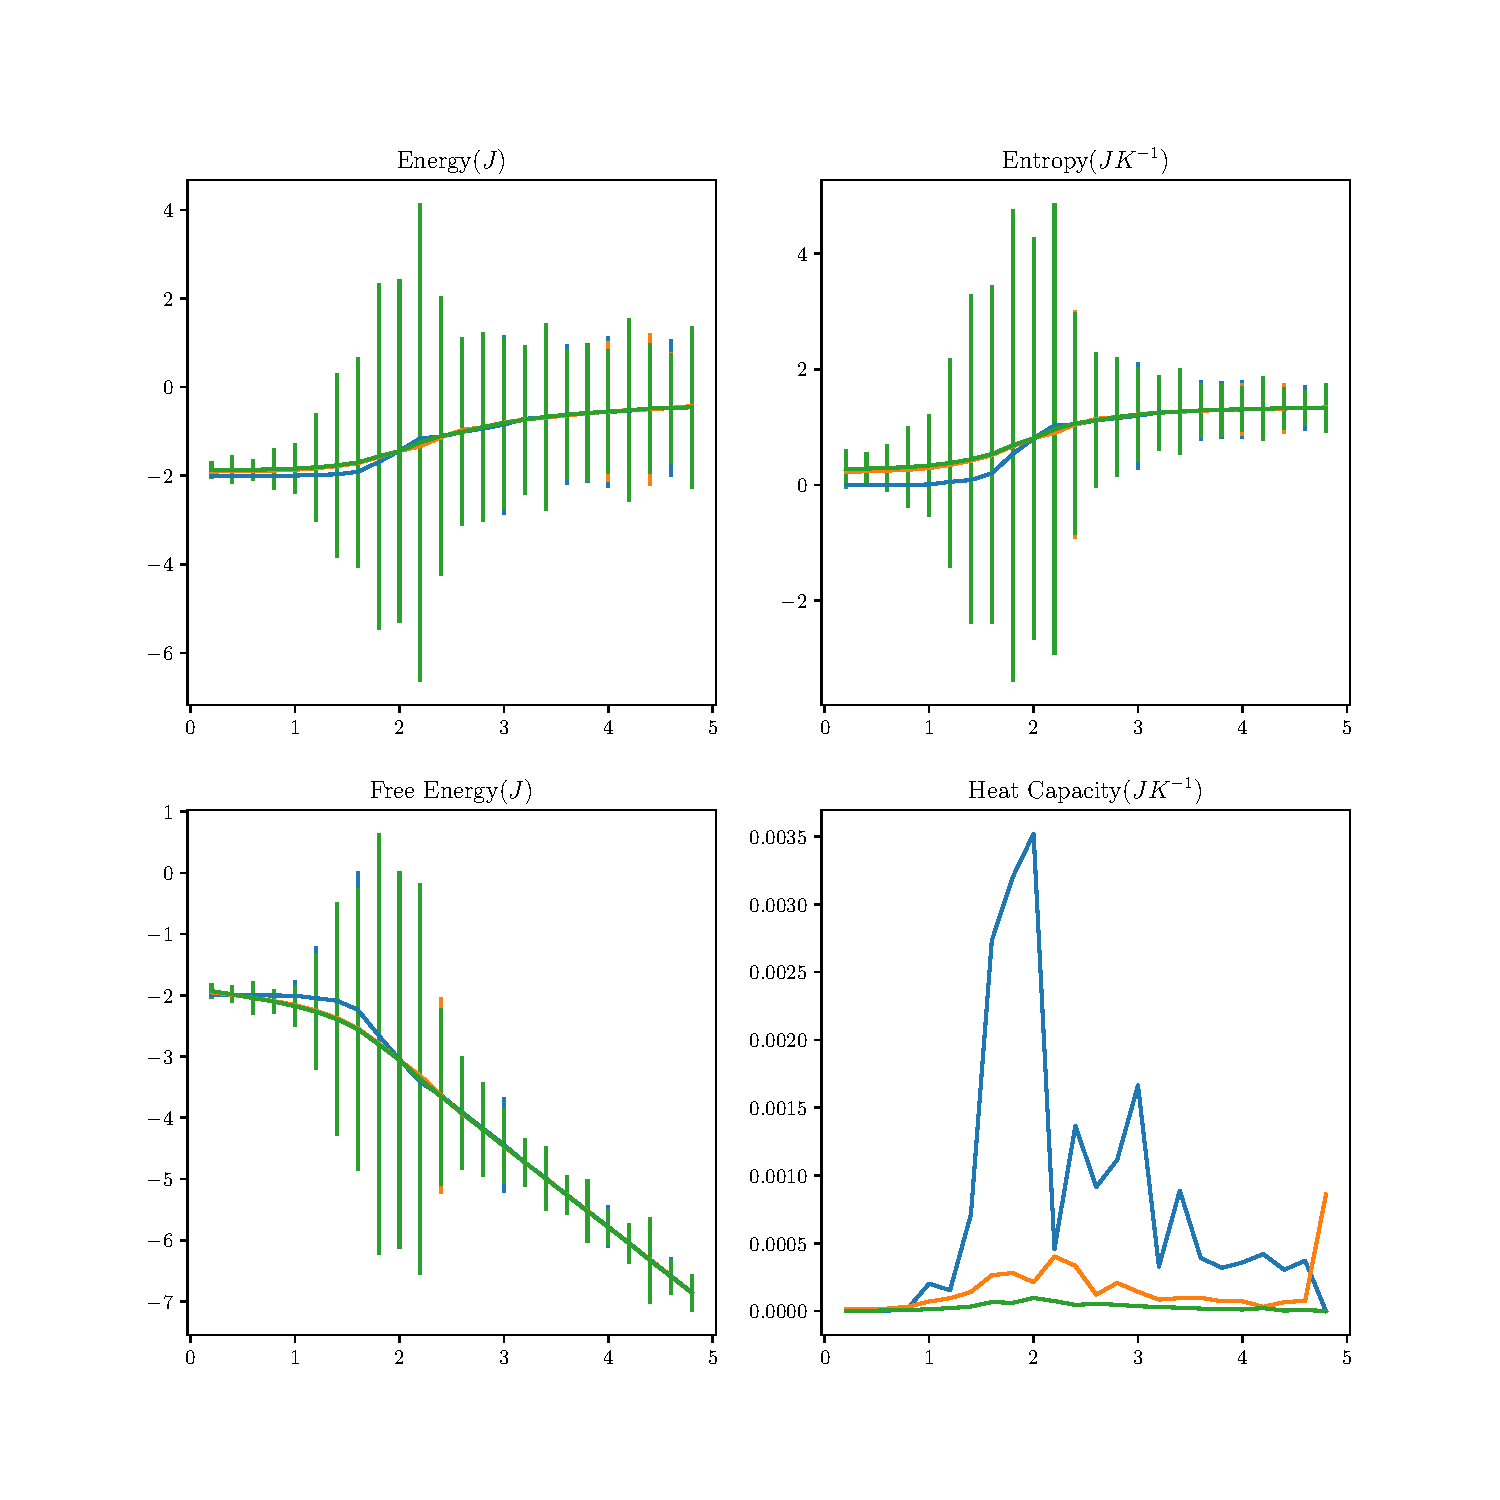
\includegraphics[width=0.45\textwidth]{pub/figures/physical_parameters_ising_2d.pdf}
    \caption{}
    \label{fig:7}
\end{figure}
I noticed that the heat capacity \emph{spike} increased in %
height as I increased the size of the crystal. This suggests %
that the infinite Ising model will have an infinitely tall %
heat capacity \emph{spike} at the critical temperature. I also %
noticed that at the critical temperature all of the physical %
parameters changed the fastest. 


This makes sense because a phase transition is loosely defined %
as a sudden discontinuity in the bulk properties of the sample. %
Although the entropy and energy are not discontinuous over the %
the critical temperature they do change very suddenly. The %
discontinuity is in the heat capacity which is the derivative %
of the energy with respect to temperature. Because a derivative %
is the discontinuous quantity it implies that the phase transition %
is second order. 


To measure the energy of the two dimensional Ising system I %
used a very similar piece of code to the one dimensional %
scenario. 

\begin{lstlisting}
/*
 * energy_ising_t
 * --------------
 * Calculate the energy of the 
 * Ising system. 
 *
 * parameters
 * ----------
 * ising_t *system: The system to 
 *     measure. 
 */
float energy(ising_t *system)
{
    int length = system->length;
    int **ensemble = system->ensemble;
    float epsilon = system->epsilon;
    float field = system->magnetic_field;
    float magnetic = 0.0;
    float interactions = 0.0;

    for (int row=0; row<length; row++)
    {
        for (int col=0; col<length; col++)
        {
            float neighbours = 
                ensemble[modulo(row+1,length)][col] +
                ensemble[modulo(row-1,length)][col] +
                ensemble[row][modulo(col+1,length)] +
                ensemble[row][modulo(col-1,length)];

            magnetic -= ensemble[row][col] * 
                field;
            interactions -= neighbours * 
                epsilon * ensemble[row][col];
        }
    }

    return interactions / 2. + magnetic;
}
\end{lstlisting}

For the entropy the calculation was also very similar. 

\begin{lstlisting}
/*
 * entropy_ising_t
 * --------------
 * Calculate the entropy of the Ising 
 * system. 
 *
 * parameters
 * ----------
 * ising_t *system: The system to 
 *     measure. 
 */
float entropy_ising_t(ising_t *system)
{
    int len = system->length;
    int **ensemble = system->ensemble; 
    int up = 0;

    for (int row=0; row<len; row++)
    {
        for (int col=0; col<len; col++)
        {
            up += ensemble[row][col] == 
                ensemble[modulo(row+1,len)][col];
            up += ensemble[row][col] == 
                ensemble[row][modulo(col+1,len)];
        }
    }
        
    int total = 2 * len * len;
    int down = total - up;

    return total * log(total) - 
        up * log(up) - down * log(down);
}
\end{lstlisting}


\subsection*{Question 2 d)}
\begin{figure}
    \centering
    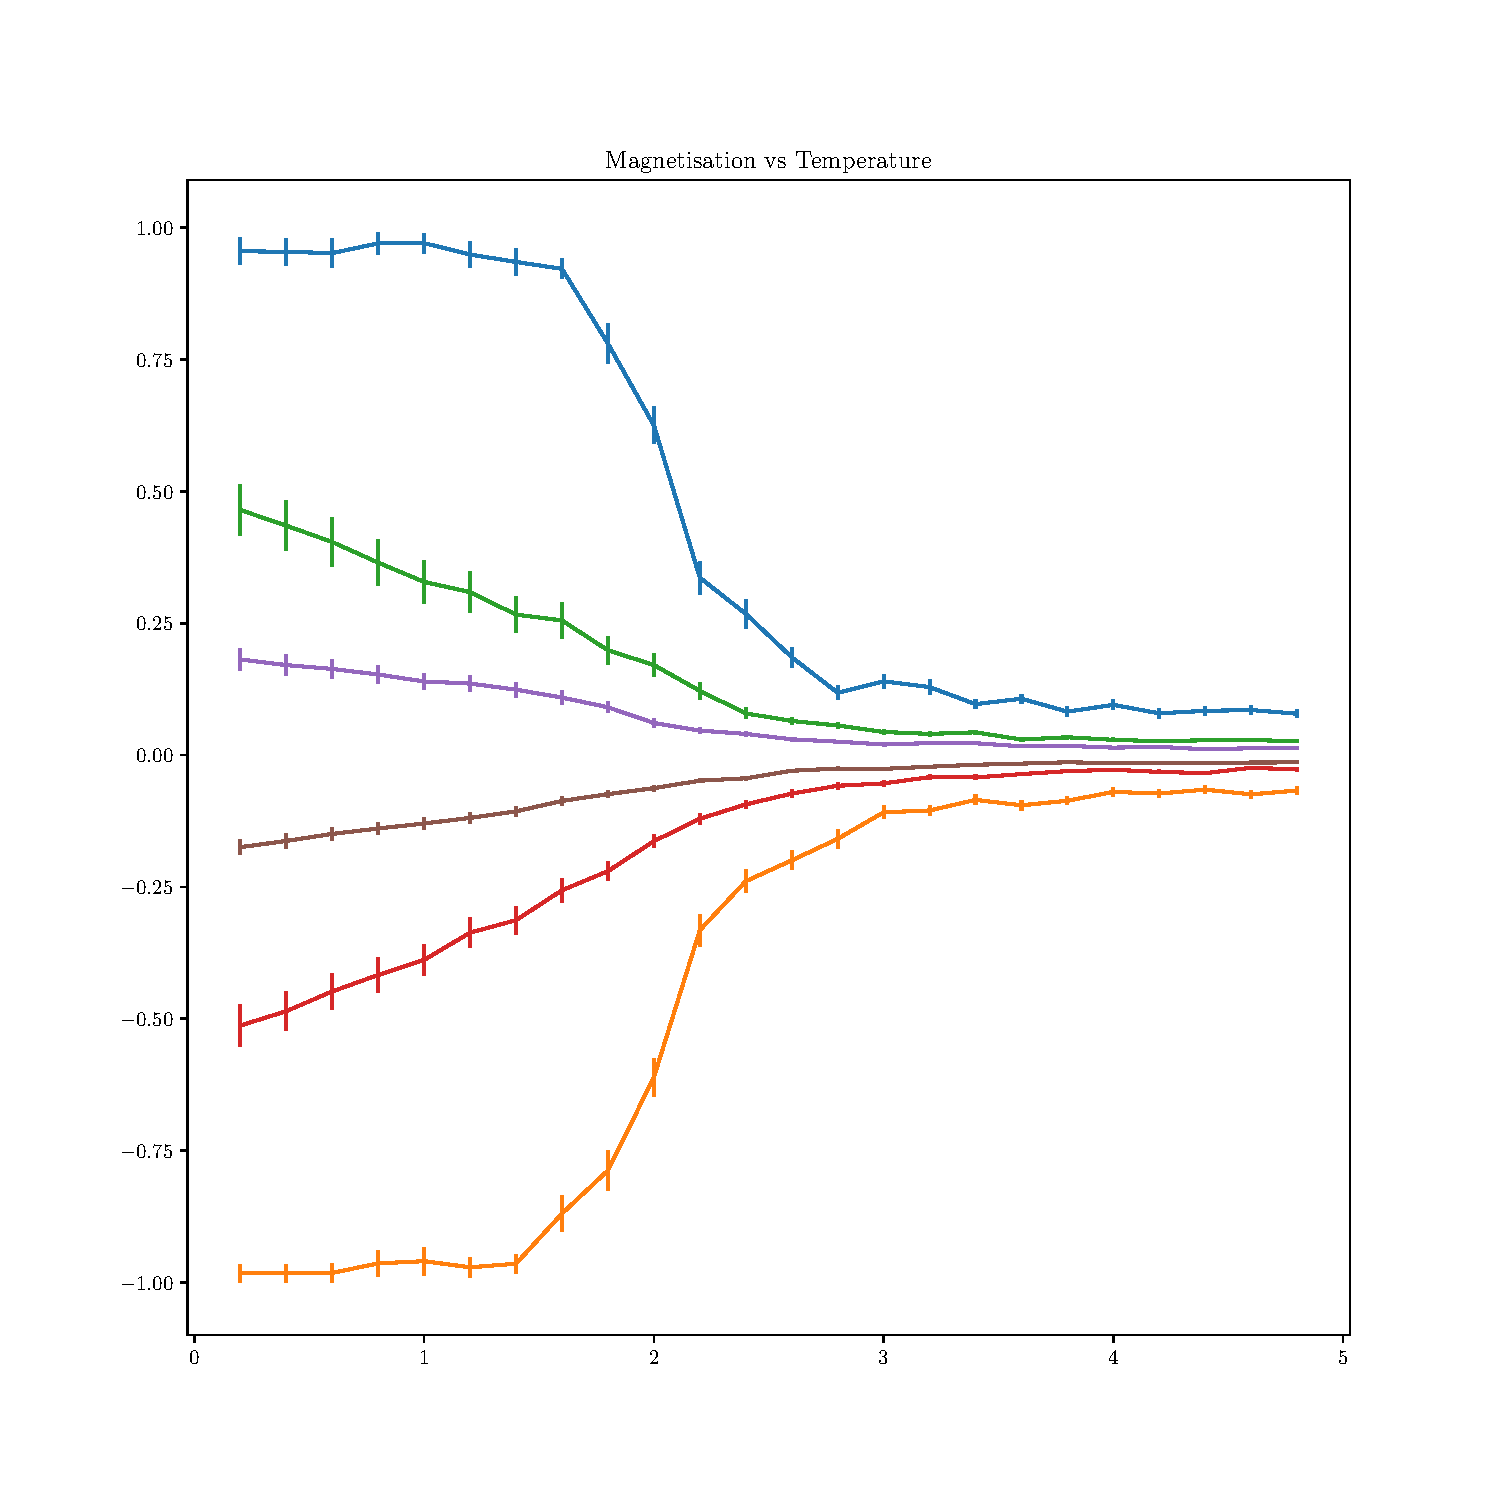
\includegraphics[width=0.45\textwidth]{pub/figures/magnetisation_ising_2d.pdf}
    \caption{The magnetisation of the Ising model as the %
        temperature and number of spins is varied.}
    \label{fig:8}
\end{figure}


I noticed that the magnetisation began to diverge at the same %
temperature irrespective of the size of the system. This is what %
I would expect from a phase transition because it should not depend %
on the size of the sample. To give a real world example iron melts %
at the same temperature regardless of the size of the block. %
We might more quickly melt a smaller block but that is just because %
there is less of it and less self insulation. 


As \(N\) increases the critical temperature will stay the same, %
but the steepness of the transition appears to radically increase. %
I was surprised to see this relationship and I believe it may %
be because we are at the very low number end of the spectrum. %
In this regime if one or two spins flip it becomes visible on %
the graph. What I expect to see is that the lines smoothly %
converge down to a step function at the critical temperature. 


\subsection*{Question 2 e)}
\begin{figure}
    \centering
    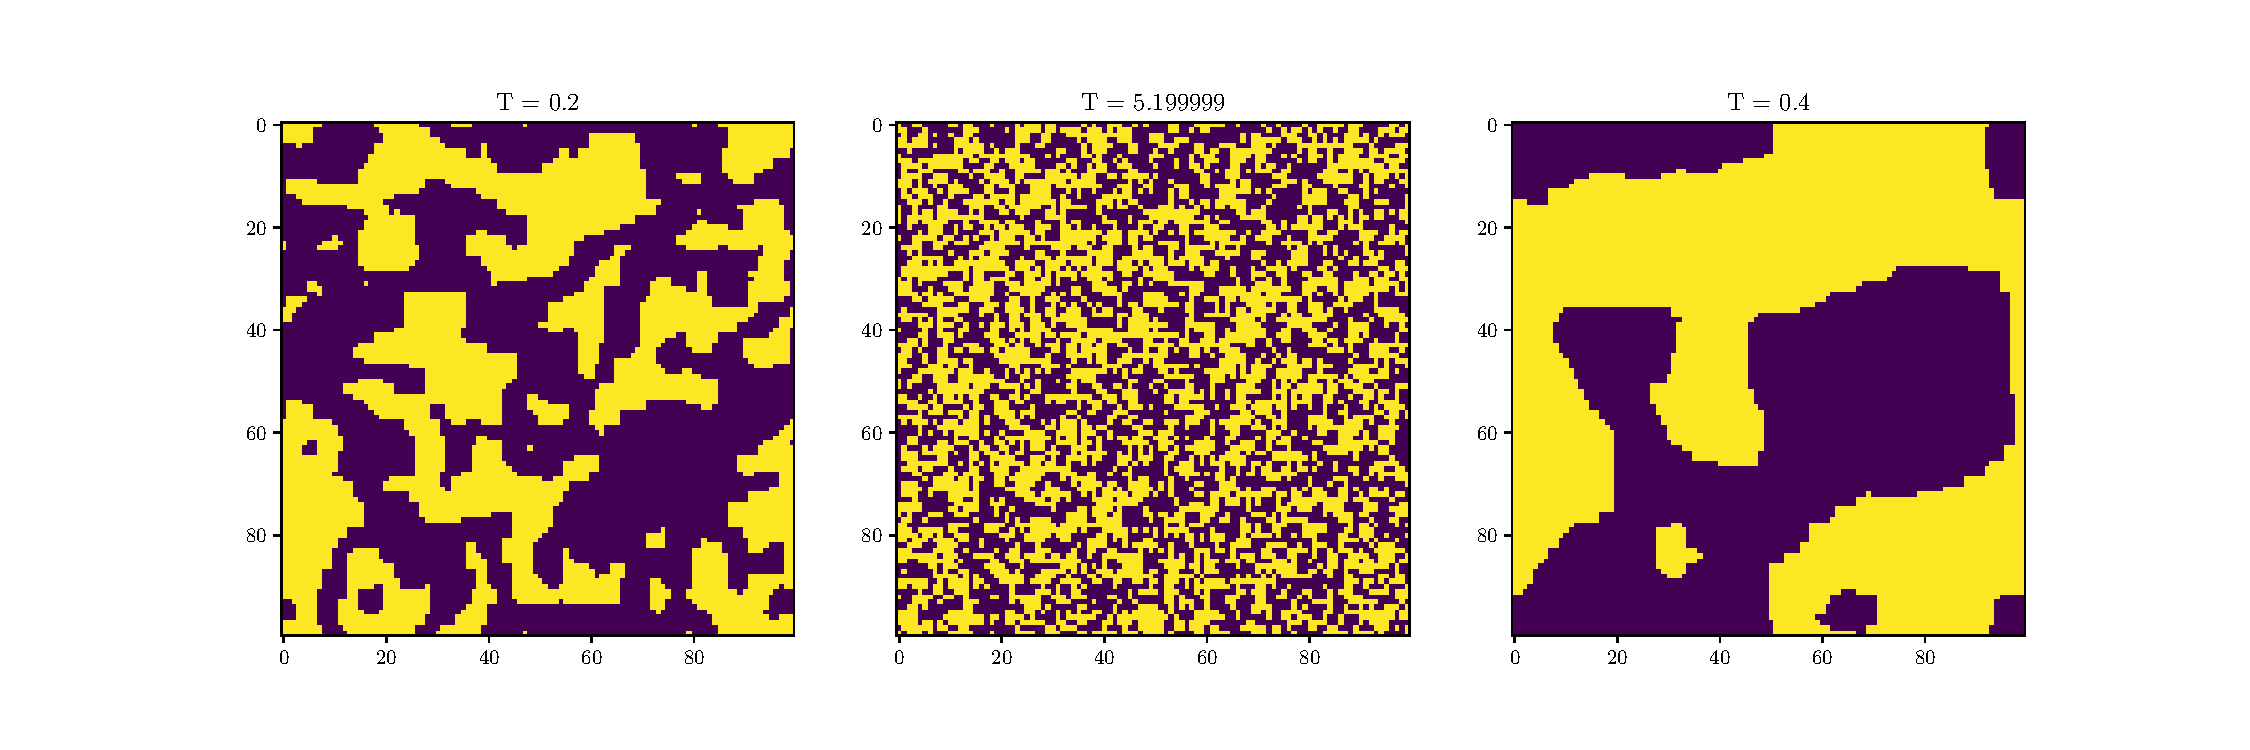
\includegraphics[width=0.45\textwidth]{pub/figures/heating_and_cooling_ising_2d.pdf}
    \caption{Heating and cooling an Ising system to change the %
        magnetisation. The leftmost figure is the initial state %
        at the lowest temperature, the middle figure is the highest %
        temperature state and the rightmost figure is the final %
        final state after the system has again been cooled.}
    \label{fig:9}
\end{figure}

I initialised the system randomly. This corresponds to the %
equilibrium of a system that is at a high temperature. %
Therefore, I first cooled the system to reach an equilibrium %
that I would expect for a low temperature state. This was done %
slowly letting the system equilibrate at each new temperature. %
This technique avoids the \emph{meta-stable} rings from forming. 


The cooled system represents the leftmost figure in \ref{fig:9}. %
We can see that the magnetisation is complete and in this case %
there are not even any speckles. This is suspiciously good but %
I cannot find the error in my code so I will run with it. At %
the highest temperature we see that the state appears to be %
almost entirely random. Cooling it back down I managed to get %
a \emph{meta-stable} ring state.


In all the heating and cooling operations I raised the temperature %
slowly and re-equilibrated the system at each new temperature. %
I am annoyed by the ring state because this gradual cooling is %
supposed to prevent such states for the most part. Again this %
state is markedly non-speckled and I think this is because the %
temperature is very close to \(0.0 \epsilon / k\). We also see %
that the edges of the ring are pixel flat. 


I justify this because the corners are where the \emph{domains} %
die as I discussed above. Hence any incursion that yellow makes %
into the purple band is unstable because the incurring yellow %
are more likely to have purple neighbours than yellow neighbours. %
The same can be said for the purple incursions into yellow %
territory. Therefore, by far the most stable configuration is %
the flat edged band which we observe. 


The final thing I want to discuss is the change in the magnetisation %
of the system between the first cool state and the final cool state. %
We can see that the injection of thermal energy into the system %
has changed the magnetisation from purple to predominantly yellow %
ignoring the \emph{meta-stable} ring. 


The Currie temperature is defined as the temperature at which the %
magnetic properties of a metal change dramatically. Since this is %
the behaviour that we are observing at the critical temperature %
it makes sense that the critical temperature is analogous to the %
Curie temperature. In the briefing %
we were given that the critical temperature for the two dimensional %
Ising model was \(T_{c} \approx 2.27\epsilon / k\). The Curie %
temperature of iron is \(T_{c} = 1043K\), hence \(\epsilon = %
1043K * k / 2.27 = 0.0396eV\). 
\vfill


\clearpage
\section*{Introduction}
The study of magnetic materials is an area of academic %
and industrial interest \cite{Shroeder2021}. For example, magnetic %
technologies are important in the ongoing development of %
quantum computers, superconducting circuits and other %
examples in electronics. At a fundamental level %
magnetisation is a well understood phenomenon, yet it is %
difficult to theoretically model. One simple model of magnetic %
materials is the Ising model. 


The Ising model is a simple model of a ferro-magnet \cite{MacKay2003}. %
Despite the simplicity of the Ising model it displays rich %
physical behaviour and has analytic solutions in one and %
two dimensions \cite{MacKay2003, Schroeder2021}. The Ising model is the %
simplest model to account for inter-molecular interactions and contain a phase %
transition. This makes it an excellent medium for studying %
magnetic phenomenon \cite{MacKay2003}. 


By modifying the basic Ising model we can simulate many %
phenomenon including glasses \cite{McMillan1984}. The Ising model %
has broader significance and can be used to construct very %
simple neural networks called Boltzmann machines \cite{MacKay2003}. We %
used the Ising model to compare ferro-magnetic, para-magnetic and %
anti-ferro-magnetic materials. Iron is a good example of a material %
that is ferro-magnetic, whereas gold is para-magnetic and chromium %
is anti-para-magnetic. 


\section*{Theory}
Materials have internal interactions. As physicists we like %
to ignore these where possible but often these approximations %
limit the accuracies of our models \cite{Schroeder2021, Kittel1969}. Magnetic %
phenomenon are no different. To understand how spins interact %
in a magnet it helps to first construct the simplest possible %
model without interactions; a para-magnet.


Consider our magnet as a one-dimensional chain of atomic spins. %
For the moment ignore any external magnetic field and just %
consider the spins in isolation. Now lets limit the spins to %
be fixed up or down along one axis. If there are no interactions %
between the spins the energy is fixed. If we add an external %
magnetic field then we would expect the ensemble to develop a %
net magnetisation.


If the system has thermal energy we would expect some of the %
spins to align themselves anti-parallel to the magnetic field. %
We can see this affect by considering the partition function %
for a single spin in the ensemble. If the spin is aligned with %
the magnetic field then the energy is \(-sB\), where \(s\) is %
the unit of magnetisation carried by the single spin and \(B\) %
is the strength of the external magnetic field. If the spin is %
anti-aligned with the field then the energy is \(sB\). 


This is a simple two level system and the partition function %
is given by, 
%
\begin{align}
    Z &= \sum_{s = \pm 1}\exp\left(-\frac{sB}{\tau}\right)\nonumber\\
        &= \exp\left(-\frac{sB}{\tau}\right) + 
            \exp\left(\frac{sB}{\tau}\right)\nonumber\\
        &= 2\cosh\left(\frac{sB}{\tau}\right),
    \label{eqn:18}
\end{align}
%
where, \(\tau = kT\) is the temperature in units of energy. %
The probability of the spins being anti-aligned with the %
field is therefore, 
%
\begin{align}
    P &= \frac{\exp\left(-\frac{sB}{\tau}\right)}
            {2\cosh\left(\frac{sB}{\tau}\right)}.
    \label{eqn:9}
\end{align}
%
Hence, as the temperature increase we expect the number of %
anti-aligned spins to increase and as we increase the %
magnetic field we expect the number of anti-aligned spins %
to decrease. 


Since each of the spins in a para-magnetic system is independent %
the partition function of an ensemble of \(N\) spins is just %
the product of \(N\) partition functions for the single spin %
case. However, since the spins are indistinguishable we must %
also divide by a Gibbs correction factor of \(N!\). %
The energy of the system, and any other physical %
parameters, only depend on the number of spins that are %
aligned with the magnetic field and not specifically %
which spins are aligned with the field. 


It is informative to calculate the internal energy and free %
energy of the system. Starting with the internal energy,
%
\begin{align}
    U &= \tau^{2}\partial_{\tau}\ln Z\nonumber\\
        &= \tau^{2}\partial_{\tau}\ln\left(2^{N}\cosh^{N}
            \left(\frac{sB}{\tau}\right)\right)\nonumber\\
        &= -NsB\tanh\left(\frac{sB}{\tau}\right).
    \label{eqn:10}
\end{align}
%
We can also calculate the free energy, but further calculations %
result in tedious analytical expressions so we have omitted them. %
%
\begin{align}
    F &= -\tau\ln Z\nonumber\\
        &= -\tau\ln\left(2^{N}\cosh^{N}\left(\frac{sB}{\tau}
            \right)\right)\nonumber\\
        &= -NsB - N\tau\ln\left(1 + \exp\left(-\frac{2sB}{\tau}\right)
            \right).
    \label{eqn:11}
\end{align}
%
Curiously this matches with the results we found for the Ising %
model when there was no magnetic field. Using %
equation \ref{eqn:5} we can calculate the magnetisation as a function %
of the magnetic field and temperature, 
%
\begin{align}
    U = mB &= -NsB\tanh\left(\frac{sB}{\tau}\right)\nonumber\\
        m &= -Ns\tanh\left(\frac{sB}{\tau}\right).
    \label{eqn:12}
\end{align}
%
Therefore, the net magnetisation system will decrease with %
temperature and increase with the magnetic field, much as we %
would expect. 


Para-magnets are a useful toy model but from our experience %
with natural and manufactured magnets we know that it is %
possibe to construct systems that are magnetic without external %
fields. The one-dimensional Ising model is a simple model of %
such systems. The Ising model is a natural extension of the %
paramagnetic model that we discussed, and operates on the same %
spin lattice. 


The Ising model differs because it adds very simple interactions %
between neighbouring spins. This interaction favours pairs that %
are aligned by reducing the energy of this scenario. Representing %
up spins as \(+1\) and down spins as \(-1\) we can represent this %
mutual interaction as \(\Delta U = \epsilon s_{i}s_{i + 1}\), %
where \(\Delta U\) is the energy contribution of the %
interaction, \(\epsilon\) is a scaling factor that represents %
the strength of the interaction and \(s_{i}\) is the \(i^{th}\) %
spin in the chain. 


What happens if we place the Ising model into an external magnetic %
field. Again we can break it down by considering a single pair %
in the chain as our constituent object. There are three energies %
that it is possible for this pair to have; parallel and aligned %
with the magnetic field, parallel and anti-aligned with the %
magnetic field and anti-parallel. However, the final state has a %
multiplicity of two since either of the spins could be aligned %
with the field. 


Based on our analysis of the paramagnetic system we would expect %
that the magnetic field would coerce spins into alignment by %
decreasing there energy. This produces a positive reinforcement %
loop because now the energy of the neighbouring spin is not %
only decreased by \(sB\) when it aligns with the field but is %
also decreased by \(\epsilon s_{i}s_{i + 1}\). We predict that %
adding the external field will raise the critical temperature of %
the system. 


We expect the type of phase transition to change. In %
general the spins will be flipping much less rapidly and as %
a result the humpy in the heat capacity will be smoothed out %
because the variance in the temperature will not peak as %
largely. Since, we expect that the heat capacity will be %
continuous this implies that the type of phase transition %
is now first order, where the energy is getting provided by the %
magnetic field. 


Moreover, we expect that many of the rich behaviours we observed %
in the absence of an external magnetic field will vanish. For %
example, below the critical temperature we expect the lifetime %
of \emph{domains} to be significantly shorter as the entire %
crystal quickly condenses into the ground state. In addition, %
we expect \emph{speckling} to be even rarer and slower because %
the flip now has a weight lower be a factor of \(\exp(-sB)\). 


Another interesting effect that can be explored using the Ising model %
is anti-ferro-magnetism. This phenomenon was only recently discovered %
in nature and refers to and interaction between neighbouring %
spins that causes them to have lower energy when they are aligned %
anti-parallel rather than parallel. We do not need to cover any new %
equations in this case as an anti-ferro-magnet can be explored by %
letting \(\epsilon\) become negative. 


It is worth noting that in the presence of a magnetic field the %
qualitative behaviour of the anti-ferro-magnetic and ferro-magnetic %
Ising models becomes markedly different. The ferro-magnetic model %
results in a positive feedback loop as the magnetic field coerces %
spins to align with the field they also want to align with each other.
On the other hand the anti-ferro-magnet exerts a dampening effect %
for the opposite reason. 


\section*{Hypothesis}
We predicted that the anti-ferro-magnetic material would have a phase %
transition at the same temperature as the ferro-magnetic material in %
the absence of an external magnetic field. We came to this conclusion %
because the type of interaction is the same and all that has changed is %
the sign. The presence of an external field was expected to change %
this phase transition, which we expected to be second order based on %
the ferro-magnetic Ising model, to a first order phase transition. 


We also predicted that the phase transition of the ferro-magnetic %
Ising model would change from a second order phase transition to a first %
order phase transition in the presence of an external magnetic field. %
This prediction was based on the unequal weighting of the orientations %
reducing the variability of the energy and hence smoothing out the %
peak in the heat capacity. A corollary of this second hypothesis was %
that the magnetic field would increase the critical temperature of %
the model. 


Finally we presented a number of equations predicting how the %
para-magnetic material would evolve as the magnetic field was varied. %


\section*{Method}
We tested our the anti-ferro-magnetic phase transition hypothesis by %
measuring the physical parameters at a number of different temperatures %
and plotting the results. This allowed us to search for a suspected %
discontinuity in the heat capacity which would indicate a second order %
phase transition akin to the phase transition of the ferro-magnetic %
substance. We repeated the same thing at three different strengths of %
magnetic field noting how the peak in the heat capacity qualitatively %
changed. As a result we were able to estimate the Neel temperature of %
the lattice based on the location of the \(B = 0\) peak.


We used the same method to test how the ferro-magnetic phase transition %
was changed by the external magnetic field. However, we also tested %
increasing the strength of the magnetic field once the system was %
equilibrated below above and at the critical temperature. This gave %
us the ability to look for a similar, but not the same phase transition %
which we expected to be first order. 


To test our predictions for the paramagnetic substance we simulated it %
over a fine grid of temperatures and the same three magnetic fields as %
the other simulations. We quantitatively assessed our models by calculating %
the \(\chi^{2}\) statistics for each fit and the associated \(p\)-value. %


My original code could not be used to test these predictions so I modified %
it to accommodate the flexible \(\epsilon\) and \(B\) into the sub-routines. %
Below I have included snapshots for the energy subroutine, entropy subroutine %
and the monte-carlo step subroutine. 

\begin{lstlisting}
/*
 * metropolis_step_ising_t
 * -----------------------
 * Evolve the system according to a 
 * randomly weighted spin flip that 
 * compares the probability of the 
 * two states based on the Boltzmann 
 * distribution of the two systems. 
 *
 * parameters
 * ----------
 * ising_t *system: The system to 
 *     evolve. 
 */
void metropolis_step(ising_t *system)
{
    int length=system->length;
    int **ensemble=system->ensemble;
    float epsilon=system->epsilon;
    float temp=system->temperature;
    float field=system->magnetic_field;

    int row = random_index(length);
    int col = random_index(length);

    int spin = ensemble[row][col];
    int neighbours = 
        ensemble[modulo(row+1,length)][col]+
        ensemble[modulo(row-1,length)][col]+
        ensemble[row][modulo(col+1,length)]+
        ensemble[row][modulo(col-1,length)];

    float magnetic=2*spin*field;
    float interaction=2*epsilon*
        neighbours*spin;
    float change=magnetic+interaction;

    if ((change<0) || 
        (exp(-change/temp)>randn()))
    {
        ensemble[row][col]*=-1;
    }
}
\end{lstlisting}


\begin{lstlisting}
/*
 * energy_ising_t
 * --------------
 * Calculate the energy of the Ising 
 * system. 
 *
 * parameters
 * ----------
 * ising_t *system: The system to measure. 
 */
float energy_ising_t(ising_t *system)
{
    int len=system->length;
    int **ensemble=system->ensemble;
    float epsilon=system->epsilon;
    float field=system->magnetic_field;
    float magnetic=0.0;
    float interactions=0.0;

    for(int row=0;row<len;row++)
    {
        for(int col=0;col<len;col++)
        {
            float neighbours = 0.0;
            neighbours+=
                ensemble[modulo(row+1,len)][col]+
                ensemble[modulo(row-1,len)][col]+
                ensemble[row][modulo(col+1,len)]+
                ensemble[row][modulo(col-1,len)];

            magnetic-=ensemble[row][col]*field;
            interactions-=neighbours*epsilon*
                ensemble[row][col];
        }
    }

    return interactions / 2. + magnetic;
}
\end{lstlisting}


\begin{lstlisting}
/*
 * entropy_ising_t
 * --------------
 * Calculate the entropy of the Ising 
 * system. 
 *
 * parameters
 * ----------
 * ising_t *system: The system to 
 *     measure. 
 */
float entropy_ising_t(ising_t *system)
{
    int len=system->length;
    int **ensemble=system->ensemble;
    int up=0;

    for(int row=0;row<len;row++)
    {
        for(int col=0;col<len;col++)
        {
            up += 
                ensemble[row][col]==
                ensemble[modulo(row+1,len)][col]+
                ensemble[row][col]==
                ensemble[row][modulo(col+1,len)];
        }
    }
        
    int total=2*len*len;
    int down=total-up;

    return total*log(total)-up*log(up)-
        down*log(down);
}
\end{lstlisting}


\section*{Results}
\begin{figure}[h]
    \centering
    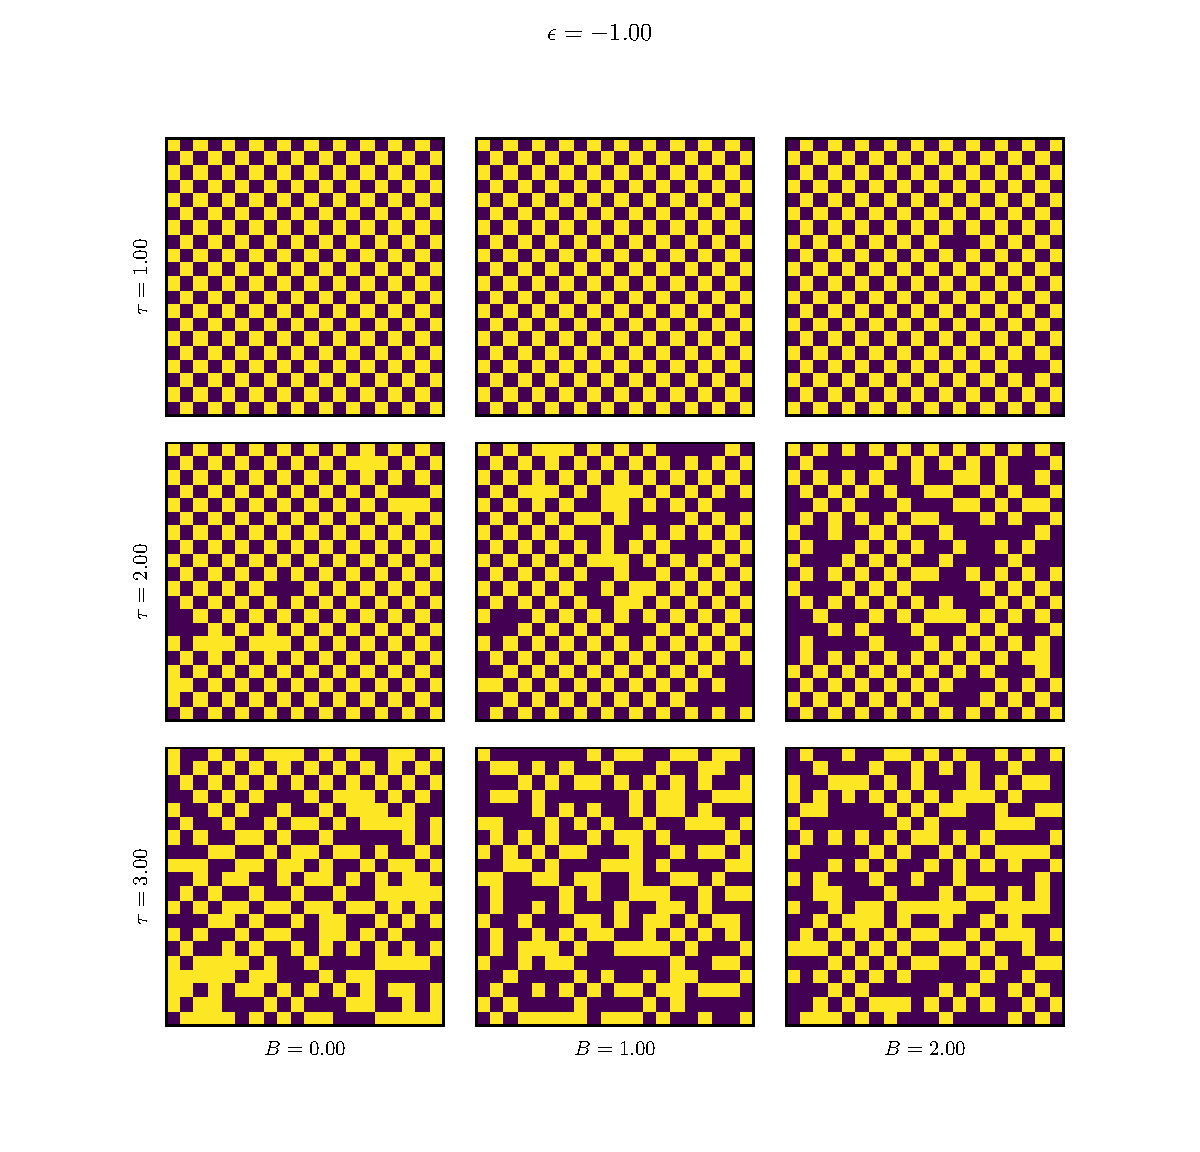
\includegraphics[width=0.45\textwidth]{pub/figures/external_field_epsilon_minus_one.pdf}
    \caption{}
    \label{fig:8}
\end{figure}


\begin{figure}[h]
    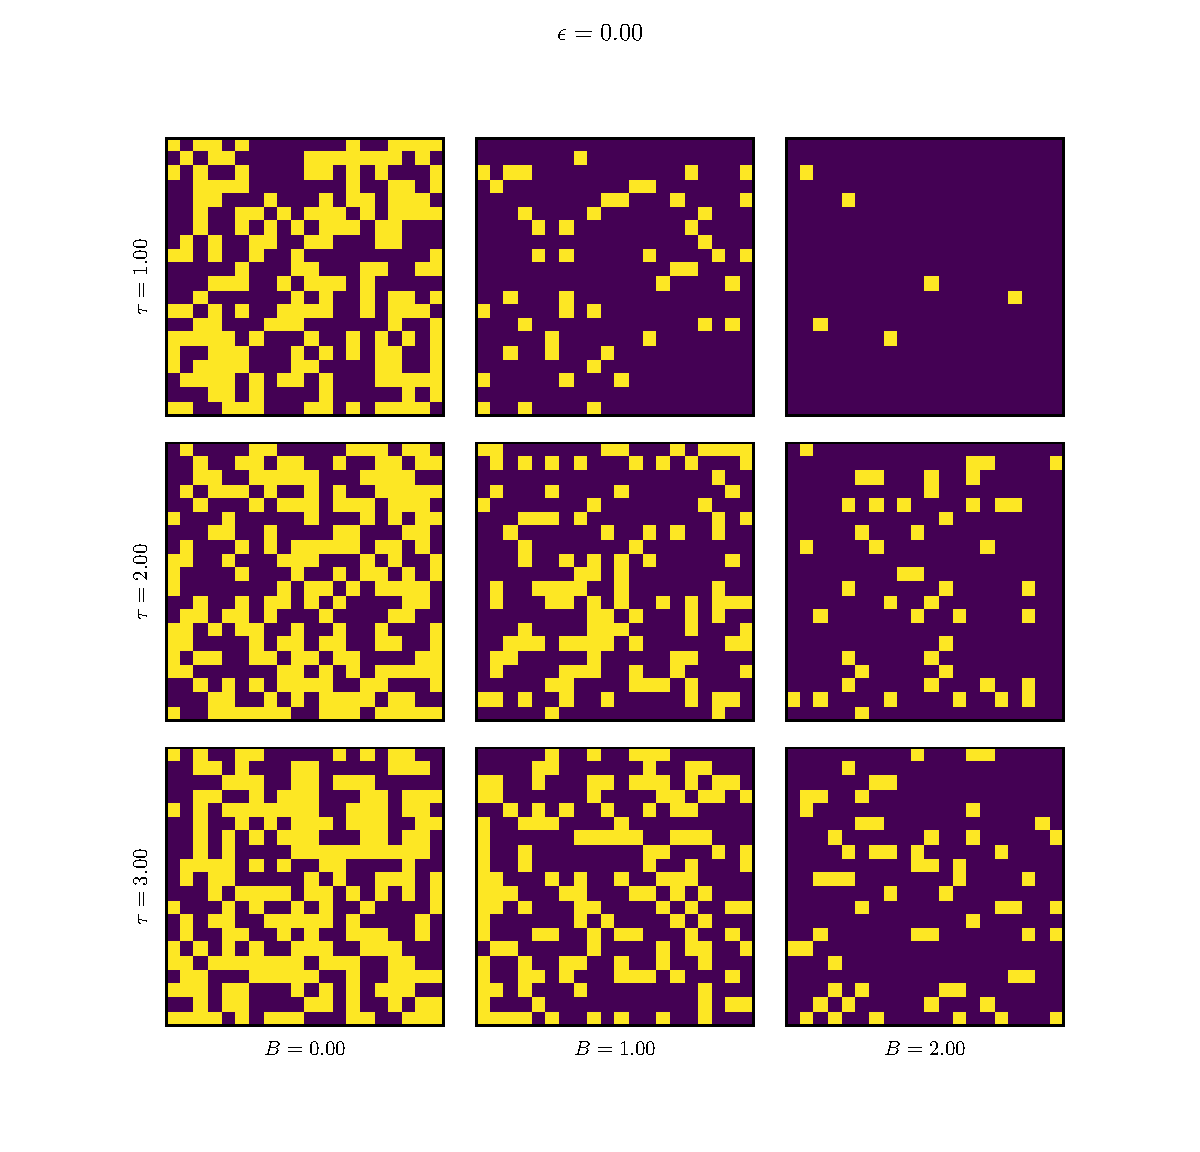
\includegraphics[width=0.45\textwidth]{pub/figures/external_field_epsilon_zero.pdf}
    \caption{}
    \label{fig:9}
\end{figure}


\begin{figure}[h]
    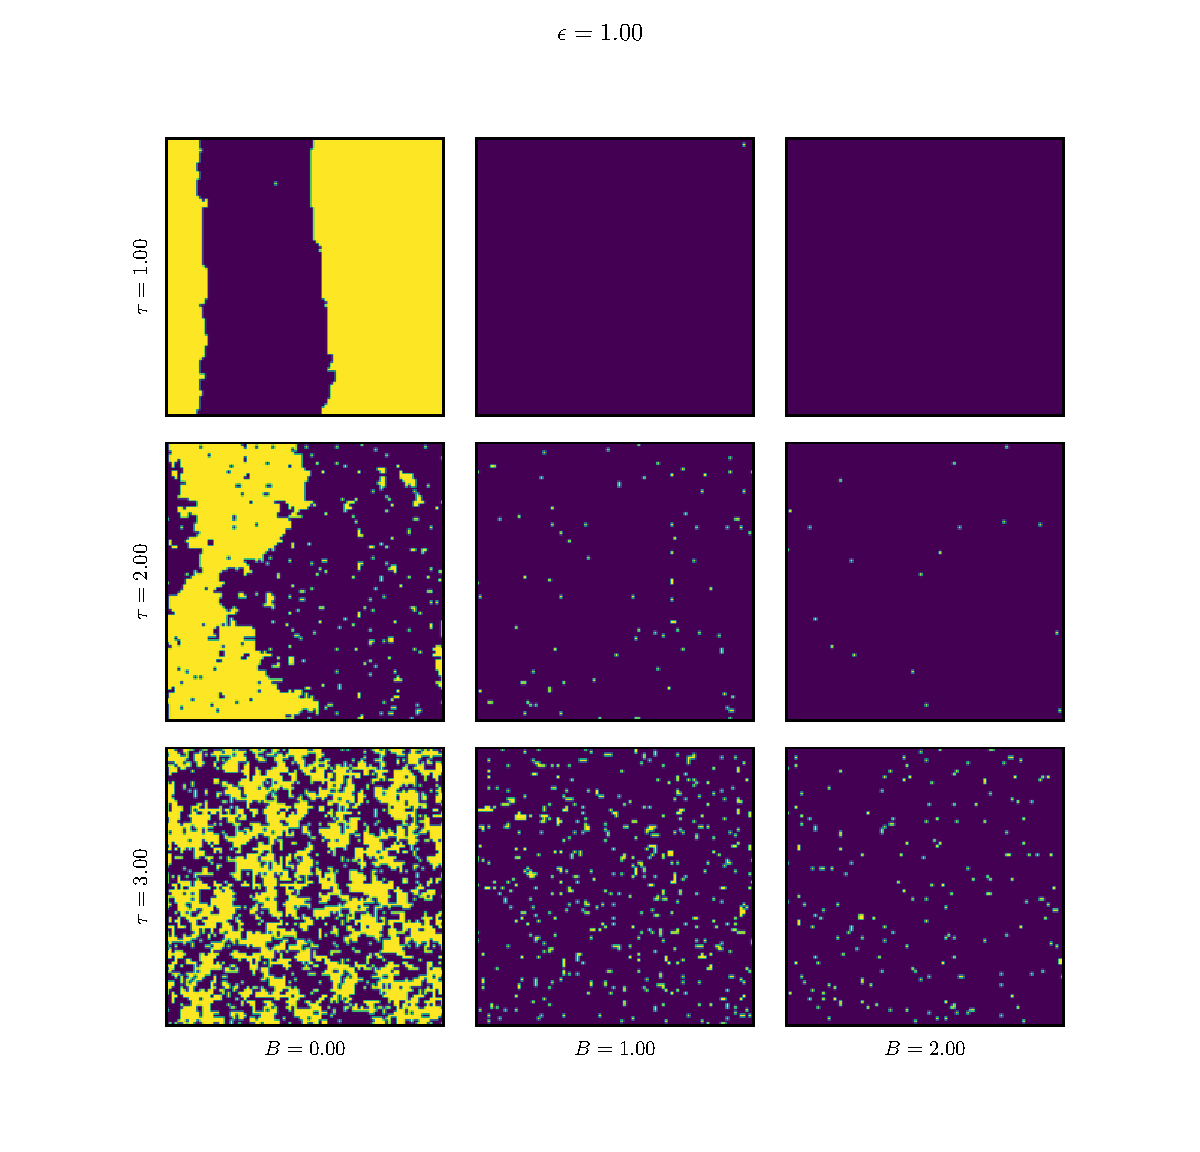
\includegraphics[width=0.45\textwidth]{pub/figures/external_field_epsilon_one.pdf}
    \caption{}
    \label{fig:10}
\end{figure}


\end{document}
